\section{Modelación}
\subsection{Bernoulli}
La ecuación de Bernoulli representa el principio de conservación de la energía para un flujo incompresible, no viscoso y estacionario. Se obtiene aplicando la Segunda Ley de Newton a un elemento diferencial de fluido a lo largo de una línea de corriente.

\begin{figure}[ht]
  \begin{center}
    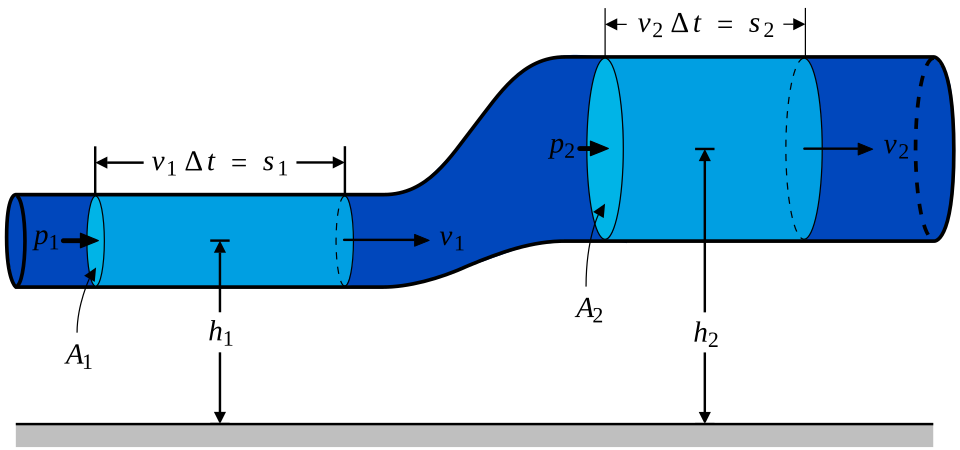
\includegraphics[width=0.8\textwidth]{figures/bernoulli.png}
  \end{center}
  \caption{}\label{bernoulli}
\end{figure}

Consideremos un elemento de fluido de sección transversal $dA$, longitud $ds$, densidad $\rho$ y masa $dm = \rho \, dA \, ds$. Las fuerzas que actúan sobre este elemento son la presión ($p$) en sus caras y la componente del peso debido a la gravedad ($g$).

Aplicando la Segunda Ley de Newton ($F = ma$) en la dirección del movimiento ($s$):
\begin{equation}
  p \, dA - (p + dp) \, dA - (\rho \, dA \, ds) \, g \sin(\theta) = (\rho \, dA \, ds) \cdot a_s
  \label{eq:fuerzas_bernoulli}
\end{equation}

Donde $p\,dA$ es la presión del lado izquierdo del fluido y $(p+dp)\,dA$ representa la variación de presión resultante de la oposición del fluido a la presión. $\theta$ es el ángulo de inclinación respecto a la horizontal. Dado que $dh = ds \sin(\theta)$, podemos reescribir la componente del peso. Además, la aceleración tangencial para un flujo estacionario es $a_s = v \frac{dv}{ds}$. Simplificando la sección $dA$:

\begin{equation}
  -dp - \rho g \, dh = \rho \, v \, dv
  \label{eq:bernoulli_dif}
\end{equation}

Dividiendo por la densidad $\rho$ y reordenando los términos:
\begin{equation}
  \frac{dp}{\rho} + v \, dv + g \, dh = 0
  \label{eq:bernoulli_int}
\end{equation}

Integrando a lo largo de la línea de corriente, y asumiendo que $\rho$ es constante (fluido incompresible), se obtiene la forma clásica de la ecuación de Bernoulli:

\begin{equation}
  P + \frac{\rho v^2}{2} + \rho g \, h = \text{constante}
  \label{eq:bernoulli_final}
\end{equation}

Luego, volviendo a ver la figura \ref{bernoulli}, es posible aplicar la ecuación \ref{eq:bernoulli_final}:
\begin{align*}
  P_1 + \frac{\rho v_1^2}{2} + \rho g \, h_1 &= \text{constante 1}
  \\[2ex]
  P_2 + \frac{\rho v_2^2}{2} + \rho g \, h_2 &= \text{constante 2}
\end{align*}

Dado que el fluido es ideal (incompresible y sin viscosidad) y el flujo es estacionario, el trabajo realizado por las fuerzas de presión se traduce íntegramente en cambios de energía cinética y potencial. Por lo tanto, la constante es la misma para cualquier sección de la tubería:
\begin{equation}
  P_{1} + \frac{\rho v_1^2}{2} + \rho g \, h_1 = P_2 + \frac{\rho v_2^2}{2} + \rho g \, h_2
  \label{b-final}
\end{equation}
%%%%%%%%%%%%%%%%%%%%%%%%%%%%%%%%%%%%%%%%%%%%%%%%%%%%%%%%%%%%%%%%%%%%%%%%%%%%%%%%%%%%%%%%%%%%%%%%%%%%%%%%%%%%%%%%%%%%%%%%%%%%%%%%%%%%%%%%%%%%%%%%%%%%%%%%%%%%%%%%%%%%%555
\subsection{Torricelli}
Utilizando la ecuación derivada en el apartado anterior, es posible proponer el siguiente caso.
\begin{figure}[h]
  \begin{center}
    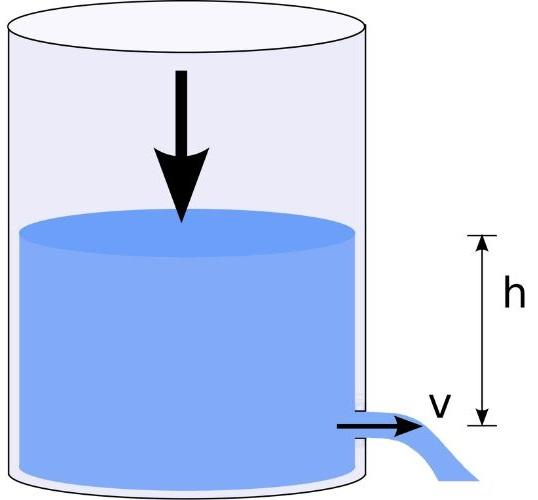
\includegraphics[width=0.45\textwidth]{figures/torricelli.jpg}
  \end{center}
  \caption{}\label{torricelli}
\end{figure}

En la figura \ref{torricelli} se muestra un sistema donde de toma $h_1$ como la altura del fluido (donde está la flecha), $h_2$ como la altura a la base del estanque, $v_1$ será la velocidad del fluido en $h_1$ y $v_2$ la velocidad del fluido en $h_2$. Aplicando la ecuación \ref{b-final} se obtiene:

$$
  P_1 + \frac{\rho 0^2}{2} + \rho g \, h_1 = P_2 + \frac{\rho v_2^2}{2} + \rho g \, 0
$$

Luego, considerando que el punto de medición de $h_2$ es fuera del estanque (donde ocurre la descarga), ambos puntos sienten la misma presión, la presión atmosférica.

$$
  P + \rho g \, h_1 = P + \frac{\rho v_2^2}{2} + 0
$$

Finalmente ordenando se tiene.

\begin{equation}
  v_2 = \sqrt{2gh_1}
  \label{Torricelli-final}
\end{equation}
%%%%%%%%%%%%%%%%%%%%%%%%%%%%%%%%%%%%%%%%%%%%%%%%%%%%%%%%%%%%%%%%%%%%%%%%%%%%%%%%%%%%%%%%%%%%%%%%%%%%%%%%%%%%%%%%%%%%%%%%%%%%%%%%%%%%%%%%%%%
\subsection{Transporte de Reynolds}
Para obtener la ecuación diferencial que describe la dinámica del nivel de agua en cada estanque, se plantea un balance de masa fundamental. 
\begin{equation}
  \frac{dm}{dt} = \dot{m}_{in} - \dot{m}_{out}
  \label{eq:balance-de-masas}
\end{equation}

Donde $\frac{dm}{dt}$ es la tasa de acumulación de masa dentro del estanque, y $\dot{m}_{in}$ y $\dot{m}_{out}$ son los flujos másicos de entrada y salida, respectivamente. Estos flujos pueden reescribirse en función de la densidad del fluido ($\rho$) y los caudales volumétricos ($Q$):

\begin{equation}
  \dot{m}_{in} = \rho Q_{in}
  \label{eq:qin}
\end{equation}

\begin{equation}
  \dot{m}_{out} = \rho Q_{out}
  \label{eq:qout}
\end{equation}

La masa total acumulada en el tanque en cualquier instante $t$ está dada por $m = \rho V$, donde el volumen $V$ es el producto del área transversal del estanque ($A$) y el nivel de líquido ($h$). Reemplazando esto en el término de acumulación se tiene:

\begin{equation}
  \frac{dm}{dt} = \frac{d(\rho A h)}{dt}
  \label{eq:acumulacion}
\end{equation}

Para simplificar el modelo y llegar a una ecuación diferencial ordinaria útil para el diseño de control, se asumen dos condiciones fundamentales del sistema físico:
\begin{enumerate}
    \item \textbf{Fluido Incompresible:} Al trabajar con agua a temperatura ambiente, se asume que la densidad $\rho$ es constante, por lo que puede salir de las derivadas y simplificarse de la ecuación general.
    \item \textbf{Geometría Cilíndrica Recta:} El área transversal del estanque $A$ es uniforme e independiente de la altura $h$, permitiendo extraerla como una constante.
\end{enumerate}

Aplicando estos supuestos, la ecuación \ref{eq:acumulacion} se reduce a $\rho A \frac{dh}{dt}$. Al sustituir todas las expresiones en la ecuación de balance (\ref{eq:balance-de-masas}) y cancelar la densidad $\rho$ a ambos lados de la igualdad, se obtiene el balance volumétrico final:

\begin{equation}
  A\frac{dh}{dt} = Q_{in} - Q_{out}
  \label{eq:balance_volumetrico}
\end{equation}

\subsection{Modelación Fenomenológica del Sensor de Nivel (Prosonic M)}

La medición de nivel en la planta se realiza mediante un transmisor ultrasónico Endress+Hauser de la familia Prosonic M. Para integrar este instrumento al lazo de control, es necesario modelar tanto su transformación estática (ganancia) como su comportamiento dinámico.

\subsubsection{Modelo Estático (Ganancia del Transmisor)}
El sensor realiza una transustanciación de la variable física (nivel de agua, $h$) a una señal eléctrica estandarizada (bucle de corriente de 4-20 mA). Asumiendo un comportamiento lineal dentro del rango de calibración, la ganancia del transmisor $K_s$ y a medición se defines como:
\begin{equation}
  h = \underbrace{h_o}_\text{distancia estanque vacío} - \underbrace{\frac{v_{sonido}\cdot \delta t}{2}}_\text{Distancia medida}
  \label{prosonic}
\end{equation}

\begin{equation}
  K_s = \frac{\text{Señal}_{max} - \text{Señal}_{min}}{h_{max} - h_{min}} = \frac{20\text{ mA} - 4\text{ mA}}{\text{Span}}
  \label{eq:ganancia_sensor}
\end{equation}

Posteriormente, en el módulo analógico del PLC ControlLogix, esta señal se escala nuevamente a unidades de ingeniería (ej. de 0 a 100\% o de 0 a 0.6 metros). Si el escalamiento en el PLC es computacionalmente exacto e inverso a la calibración del sensor, la ganancia equivalente del lazo de instrumentación puede aproximarse a $K_s \approx 1$ [m/m].

\subsubsection{Modelo Dinámico}
Aunque la propagación del sonido en el aire es sumamente rápida, la dinámica del instrumento no es instantánea. El sensor ultrasónico introduce dos efectos temporales al lazo de control:
\begin{enumerate}
    \item \textbf{Retardo de procesamiento ($t_d$):} El tiempo finito que tarda el microprocesador del sensor en emitir el pulso acústico, recibir el eco, validar el perfil de la curva de envolvente y actualizar la salida analógica de 4-20 mA.
    \item \textbf{Filtro de Amortiguación ($\tau_s$):} Para evitar que el ruido de alta frecuencia (el oleaje o turbulencia superficial del agua debido a la caída desde la bomba) genere fluctuaciones erráticas en la señal de control, los transmisores Prosonic M incorporan un filtro electrónico pasa-bajos configurable (Damping).
\end{enumerate}

Por lo tanto, la función de transferencia fenomenológica del sensor en el dominio de Laplace, que relaciona el nivel medido $H_m(s)$ con el nivel real $H(s)$, se aproxima a un modelo de primer orden con tiempo muerto (FOPDT):

\begin{equation}
  G_s(s) = \frac{H_m(s)}{H(s)} = \frac{K_s}{\tau_s s + 1} e^{-t_d s}
  \label{eq:dinamica_sensor}
\end{equation}

\textbf{Nota Operacional (Restricción Física):} Es fundamental considerar la \textit{distancia de bloqueo} (zona muerta o "blind zone") característica de estos sensores. El Prosonic M no puede medir ecos que retornen antes de que su transductor deje de vibrar por la emisión inicial. Por lo tanto, el nivel máximo operativo ($h_{max}$) del estanque debe diseñarse siempre por debajo de esta zona ciega para evitar la saturación en la lectura y la consiguiente pérdida de control del lazo.

\subsection{Modelación Fenomenológica del Sensor de Flujo (Promag 50W)}

La medición del caudal inyectado por las bombas hacia los estanques se realiza mediante un flujómetro electromagnético Endress+Hauser Promag 50W. Su principio de funcionamiento se rige por la Ley de Inducción de Faraday, donde el fluido conductivo que atraviesa un campo magnético constante ($B$) induce una fuerza electromotriz ($E$) directamente proporcional a su velocidad media ($v$):

\begin{equation}
  E = B \cdot D \cdot v
  \label{eq:faraday}
\end{equation}

Dado que el área transversal de la tubería ($A$) es constante, el caudal volumétrico es $Q = v \cdot A$. En consecuencia, la tensión inducida medida por los electrodos del instrumento es linealmente proporcional al caudal. 
\begin{equation}
  E = B \cdot D \cdot \left(\frac{Q}{A}\right) \implies Q = \frac{E \cdot A}{B \cdot D}
\end{equation}

Sabiendo que el área transversal de la tubería es $A = \frac{\pi D^2}{4}$, la expresión se simplifica a:

\begin{equation}
  Q = \left( \frac{\pi \cdot D}{4 \cdot B} \right) \cdot E
\end{equation}
\subsubsection{Modelo Estático (Ganancia)}
El transmisor del Promag 50 procesa este voltaje microscópico y lo mapea linealmente a una señal estándar de 4-20 mA. La ganancia estática del sensor $K_f$ queda definida por la parametrización de fondo de escala ($Q_{max}$) configurada en el instrumento:

\begin{equation}
  K_f = \frac{20\text{ mA} - 4\text{ mA}}{Q_{max} - 0}
  \label{eq:ganancia_flujometro}
\end{equation}

Dentro del PLC ControlLogix, esta señal se escala nuevamente para trabajar en unidades de ingeniería (ej. L/min o m$^3$/s), asumiendo una transustanciación ideal donde la ganancia aparente del lazo de instrumentación es 1.

\subsubsection{Modelo Dinámico}
A diferencia de los sensores acústicos o térmicos, el tiempo de respuesta electromagnético es virtualmente instantáneo frente a las constantes de tiempo de la planta (nivel). No existe retardo de transporte ($t_d \approx 0$) en la física de la medición.

Sin embargo, el flujo en las tuberías presenta un alto nivel de ruido de alta frecuencia debido a la turbulencia hidrodinámica y el perfil de velocidades no laminar a la salida de la bomba. Para que el lazo de control esclavo (FIC) no sature el variador de frecuencia intentando corregir este ruido, el transmisor aplica un filtro pasa-bajos electrónico (Damping o Amortiguación). Por lo tanto, la función de transferencia del sensor se aproxima a un sistema de primer orden puro:

\begin{equation}
  G_f(s) = \frac{Q_m(s)}{Q(s)} = \frac{K_f}{\tau_f s + 1}
  \label{eq:dinamica_flujo}
\end{equation}

Donde $Q_m(s)$ es el caudal medido y $\tau_f$ es la constante de tiempo del filtro configurada internamente en el Promag 50W (usualmente en el orden de décimas de segundo o pocos segundos).
\clearpage

\subsection{Modelación de planta}
\subsection{Modelo continuo}
Utilizando la ecuación \ref{eq:balance_volumetrico} se definen dos tipos de dinámicas presentes en la planta

$$
\underbrace{A\frac{dh_i}{dt}}_\text{estanque inferior} = \underbrace{\gamma_i k_i u_i + a_{i+2}\sqrt{2gh_{i+2}}}_{Q_{in}} - \underbrace{a_{i}\sqrt{2gh_{i}}}_{Q_{out}}
$$

$$
\underbrace{A\frac{dh_j}{dt}}_\text{estanque superior} = \underbrace{(1 - \gamma_j) k_j u_j}_{Q_{in}} - \underbrace{a_{j}\sqrt{2gh_{j}}}_{Q_{out}}
$$

Tal que 

\begin{align}
    A_1 \frac{dh_1}{dt} &= -a_1 \sqrt{2g h_1} + a_3 \sqrt{2g h_3} + \gamma_1 k_1 f_1 \label{eq:edo_h1} \\
    A_2 \frac{dh_2}{dt} &= -a_2 \sqrt{2g h_2} + a_4 \sqrt{2g h_4} + \gamma_2 k_2 f_2 \label{eq:edo_h2} \\
    A_3 \frac{dh_3}{dt} &= -a_3 \sqrt{2g h_3} + (1-\gamma_2) k_2 f_2 \label{eq:edo_h3} \\
    A_4 \frac{dh_4}{dt} &= -a_4 \sqrt{2g h_4} + (1-\gamma_1) k_1 f_1 \label{eq:edo_h4}
\end{align}

Donde la variable $h_i$ representa el nivel del estanque $i$, y $f_j$ corresponde a la señal de control aplicada a la bomba $j$. Los términos proporcionales a $\gamma$ y $(1-\gamma)$ reflejan la división del caudal en las válvulas.

\subsection{Discretización} % Euler

Para implementar las estrategias de control y realizar simulaciones computacionales, es necesario transformar el modelo continuo a su equivalente en tiempo discreto. Dado que los tiempos de muestreo ($T_s$) típicamente utilizados en la automatización de procesos industriales son pequeños en comparación con la constante de tiempo dominante de los estanques, el método de integración de Euler hacia adelante resulta suficiente y computacionalmente eficiente para el autómata.

Aproximando la derivada del nivel como la tasa de cambio entre dos instantes de muestreo consecutivos:
\begin{equation}
    \frac{dh(t)}{dt} \approx \frac{h[k+1] - h[k]}{T_s}
\end{equation}

Reemplazando esta aproximación en el balance de masas, se obtiene el sistema de ecuaciones en diferencias que predice el nivel en el instante futuro $[k+1]$ basándose en el estado actual $[k]$ y la acción de control actual $u[k]$:

\begin{align}
    h_1[k+1] &= h_1[k] + \frac{T_s}{A_1} \left( -a_1 \sqrt{2g h_1[k]} + a_3 \sqrt{2g h_3[k]} + \gamma_1 k_1 u_1[k] \right) \label{eq:disc_h1} \\
    h_2[k+1] &= h_2[k] + \frac{T_s}{A_2} \left( -a_2 \sqrt{2g h_2[k]} + a_4 \sqrt{2g h_4[k]} + \gamma_2 k_2 u_2[k] \right) \label{eq:disc_h2} \\
    h_3[k+1] &= h_3[k] + \frac{T_s}{A_3} \left( -a_3 \sqrt{2g h_3[k]} + (1-\gamma_2) k_2 u_2[k] \right) \label{eq:disc_h3} \\
    h_4[k+1] &= h_4[k] + \frac{T_s}{A_4} \left( -a_4 \sqrt{2g h_4[k]} + (1-\gamma_1) k_1 u_1[k] \right) \label{eq:disc_h4}
\end{align}

Estas ecuaciones discretas son la base tanto para la simulación de la planta en software externo como para la posterior deducción de los algoritmos de control digital implementados en el PLC.
    
